\documentclass[12pt]{article}
\setcounter{tocdepth}{4} %subsubsections in toc
\setlength{\parindent}{0pt} %no indent
\usepackage{mathtools}
\usepackage{physics}
\usepackage{esint} %for integrals
\usepackage{amssymb} %maths stuff%
\usepackage[dvipsnames]{xcolor} %for coloured text
\usepackage[hidelinks]{hyperref}
\usepackage[nameinlink, noabbrev]{cleveref}
%\usepackage[nottoc]{tocbibind}
\usepackage{tikz} %old figures package
\usepackage{pythonhighlight} % insert python code \begin{python}
\hfuzz=16pt
% \usepackage{siunitx} %for tables
\usepackage{import}
\usepackage{caption}
\usepackage{subcaption} %for subfigures
\usepackage{pstool}
\usepackage{xifthen}
\usepackage{pdfpages}
\usepackage{transparent}
\usepackage{graphicx}
\usepackage{scalefnt}
\usepackage[inkscapelatex=false]{svg}
\usepackage{wrapfig}
\usepackage{lmodern}
\usepackage[T1]{fontenc}
\usepackage{float}

\usepackage{sectsty} % Allows customizing section commands
\allsectionsfont{\normalfont\scshape} % Make all sections centered the default font and small caps

\usepackage{tocloft}
% Change the font for all Table of Contents entries (sections subsections etc.)
\renewcommand{\cfttoctitlefont}{\normalfont\scshape\Large}
\renewcommand{\cftsecfont}{\normalfont\scshape}
\renewcommand{\cftsubsecfont}{\normalfont\scshape}

% Change the font for page numbers in the Table of Contents
% \renewcommand{\cftpagefont}{\normalfont\scshape}

\usepackage{fancybox}
\usepackage{empheq}
\usepackage{tcolorbox} %Boxes for theorems and definitions
\tcbuselibrary{theorems}

\newtcbtheorem[number within=section]{mydef}{Definition}%
{colback=Violet!50,colframe=Blue!80!black,fonttitle=\bfseries}{def}

% Automatically add definitions to the ToC
\newcommand{\tocdef}[3]{%
\refstepcounter{subsection}
\begin{mydef}{#1}{#2}
    \addcontentsline{toc}{subsection}{\protect\numberline{\ref{def:#2}}#1}
#3
\end{mydef}
}

\usepackage[a4paper, left=20mm, right=20mm,
top=20mm, bottom=20mm]{geometry}

%\renewcommand{\figurename}{fig} %allows custom figure numbering
\renewcommand{\tablename}{Table}

\usepackage{fancyhdr} % Custom headers and footers
\pagestyle{fancyplain} % Makes all pages in the document conform to the custom headers and footers
\fancyhead{} % No page header - if you want one create it in the same way as the footers below

\fancyfoot[L]{} % Empty left footer
\fancyfoot[C]{} % Empty center footer
% \fancyfoot[R]{\thepage} % Page numbering for right footer
\renewcommand{\headrulewidth}{0pt} % Remove header underlines
\renewcommand{\footrulewidth}{0pt} % Remove footer underlines
\setlength{\headheight}{13.6pt} % Customize the height of the header

%
\makeatletter
\def\smallunderbrace#1{\mathop{\vtop{\m@th\ialign{##\crcr
$\hfil\displaystyle{#1}\hfil$\crcr
\noalign{\kern3\p@\nointerlineskip} %creates \smallunderbrace command
\tiny\upbracefill\crcr\noalign{\kern3\p@}}}}\limits}
\makeatother
%
\newcommand{\threebythree}[9]{
\begin{pmatrix}
{#1} & {#2} & {#3} \\
{#4} & {#5} & {#6} \\
{#7} & {#8} & {#9}
\end{pmatrix}
}

\newcommand{\twobytwo}[4]{
\begin{pmatrix}
{#1} & {#2}\\
{#3} & {#4}
\end{pmatrix}
}

\newcommand{\twobytwoasym}[1]{
\begin{pmatrix}
0 & {#1}\\
-{#1} & 0
\end{pmatrix}
}

\newcommand{\sym}[6]{
\begin{pmatrix}
{#1} & {#4} & {#5} \\
{#4} & {#2} & {#6} \\
{#5} & {#6} & {#3}
\end{pmatrix}
}

\newcommand{\antisym}[3]{
\begin{pmatrix}
0 & {#1} & {#2} \\
-{#1} & 0 & {#3} \\
-{#2} & -{#3} & 0
\end{pmatrix}
}
%
\newcommand{\ingen}{{\smash{\raisebox{0.5ex}{\scalebox{0.9}{G}}}\mkern -11mu \scalebox{1.5}{\text{I}}}}

\graphicspath{{images/}}

%\setcounter{chapter}{1} % Set the chapter counter to 1
\numberwithin{equation}{subsection} % Number equations within sections (i.e. 1.1 1.2 2.1 2.2 instead of 1 2 3 4)
\numberwithin{figure}{subsection} % Number figures within sections (i.e. 1.1 1.2 2.1 2.2 instead of 1 2 3 4)
\numberwithin{table}{subsection} % Number tables within sections (i.e. 1.1 1.2 2.1 2.2 instead of 1 2 3 4)

%
\newcommand{\horrule}[1]{\rule{\linewidth}{#1}} % Create horizontal rule command with 1 argument of height

%\renewcommand{\bibname}{\scalefont{.7} Bibliography}

\title{%
\normalfont \normalsize
\textsc{DIAS Computing Research Internship} \\ [25pt] % Your university school and/or department name(s)
\horrule{0.5pt} \\ [0.4cm] % Thin top horizontal rule
\huge Mercury's Magnetosphere \\ % The assignment title
\horrule{2pt} \\ [0.5cm] % Thick bottom horizontal rule
}
%
\author{O. Daniel O'Carroll\\
\small{22337259}\\
\small{\href{mailto:oocarrol@tcd.ie}{oocarrol@tcd.ie}}}
\date{\normalsize\today}
\begin{document}
%\begin{minipage}{\textwidth}
\maketitle
\tableofcontents
%\end{minipage}
%
\pagebreak
%
\section{Mercury's Magnetic Field}\label{sec:mercury_s_magnetic_field} % (fold)
%
\tocdef{Magnetic Regions}{magnetic_regions}
    {
    The regions of distinct magnetic fields are largely dictated by the \textit{solar wind}. The solar wind is a \textit{"stream"} of particles following the \textit{interplanetary magnetic field} (IMF), which is largely driven by the sun.\\

    Mercury's magnetic field is driven by currents of magma, due to the Coriolis effect, in Mercury's core that produces a magnetic field. This magnetic field is "squished" by the magnetic pressure caused by the solar wind and the IMF on the day side of the planet.
    \begin{figure}[H]
        \centering
        \includesvg[width=\linewidth]{mercury_magnetosphere.svg}
        \captionsetup{font=footnotesize}
        \caption{Diagram of Mercury's magnetic field and its interactions, showing the regions of the solar wind, magnetosheath, and magnetosphere.}
        \label{figmercurymagnetosphere}
    \end{figure}
    %
    }
%
%
\tocdef{Local Time}{local_time}
    {
        Positional value telling you Mercury's \textit{orientation} with respect to the sun i.e 12 pm noon, is facing the sun and 12 am midnight is facing away. (\textbf{Ask what this is relative to}).
    }
%
%
\tocdef{Reconnection \& the Dungey Cycle}{reconnection__the_dungey_cycle}
    {
    Reconnection is the process of energy transfer between the day-side of Mercury's magnetosphere, its night-side and the IMF. It refers to the process of magnetic field lines of the IMF and Mercury's magnetic field, breaking away and joining together. This leads to flux transfer events (FTE) where the magnetic field lines \textit{reconnect} on the night-side of Mercury. This causes the Northern lights on Earth.
    \begin{figure}[H]
        \centering
        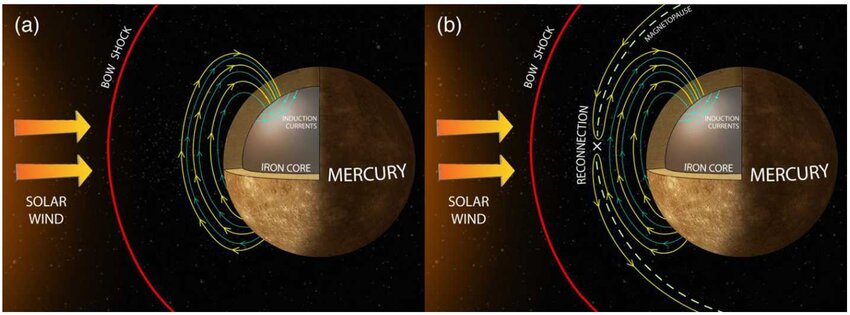
\includegraphics[width=\linewidth]{reconnection.jpg}
        \captionsetup{font=footnotesize}
        \caption{Reconnection happening on Mercury. The point where reconnection begins is called the X-line.}
        \label{figreconnection}
    \end{figure}
    %
    The \textit{Dungey cycle} is the timescale in which reconnection happens for a given system, on the order of minutes to hours.
    }
%
%
\tocdef{Parker Spiral}{parker_spiral}
    {
    The "bunging up" of the sun's magnetic field lines due to its spin.
    }
%
%
\tocdef{Satellite Motion Terminology}{satellite_motion_termninology}
    {
       \begin{center}
           \begin{tabular}{ccc|c}
               \hline
               Solar Wind & $\rightarrow$ & Magnetosheath & Bow shock in (BS\_IN)\\
               Magnetosheath & $\rightarrow$ & Solar Wind & Bow shock out (BS\_OUT)\\

                             & & &\\

               Magnetosheath & $\rightarrow$ & Magnetosphere & Magnetopause in (MP\_IN)\\
                Magnetosphere & $\rightarrow$ & Magnetosheath & Magnetopause out (MP\_OUT)
           \end{tabular}
           \label{tabmagnetopuaseandbowshock}
       \end{center}
       \textbf{Always relative to magnetic field of Mercury}.
    }
%
% section Mercury's Magnetic Field (end)
\section{Coding (hermpy) \& Data}\label{sec:coding_hermpy_} % (fold)
%
\tocdef{}{}
    {
    
    }
%
% section Coding (hermpy) (end)
\end{document}
